% !TEX TS-program = pdflatex
% !TEX encoding = UTF-8 Unicode

% This file is a template using the "beamer" package to create slides for a talk or presentation
% - Giving a talk on some subject.
% - The talk is between 15min and 45min long.
% - Style is ornate.

% MODIFIED by Jonathan Kew, 2008-07-06
% The header comments and encoding in this file were modified for inclusion with TeXworks.
% The content is otherwise unchanged from the original distributed with the beamer package.

\documentclass{beamer}

\usepackage{graphicx}

% Copyright 2004 by Till Tantau <tantau@users.sourceforge.net>.
%
% In principle, this file can be redistributed and/or modified under
% the terms of the GNU Public License, version 2.
%
% However, this file is supposed to be a template to be modified
% for your own needs. For this reason, if you use this file as a
% template and not specifically distribute it as part of a another
% package/program, I grant the extra permission to freely copy and
% modify this file as you see fit and even to delete this copyright
% notice. 


\mode<presentation>
{
  \usetheme{Warsaw}
  % or ...

  \setbeamercovered{transparent}
  % or whatever (possibly just delete it)
}


\usepackage[english]{babel}
% or whatever

\usepackage[utf8]{inputenc}
% or whatever

\usepackage{times}
\usepackage[T1]{fontenc}
% Or whatever. Note that the encoding and the font should match. If T1
% does not look nice, try deleting the line with the fontenc.


\title[Team Reverwesome: Othello Bot] % (optional, use only with long paper titles)
{COMP3130 Othello Project}

\subtitle
{Team Reverwesome} % (optional)

\author[Josh Godsiff, Jarrah Bloomfield] % (optional, use only with lots of authors)
{~Josh Godsiff \and ~Jarrah Bloomfield}
% - Use the \inst{?} command only if the authors have different
%   affiliation.

\date[Short Occasion] % (optional)
{May 29th, 2012}

% If you have a file called "university-logo-filename.xxx", where xxx
% is a graphic format that can be processed by latex or pdflatex,
% resp., then you can add a logo as follows:

% \pgfdeclareimage[height=0.5cm]{university-logo}{university-logo-filename}
% \logo{\pgfuseimage{university-logo}}


% If you wish to uncover everything in a step-wise fashion, uncomment
% the following command: 

%\beamerdefaultoverlayspecification{<+->}


\begin{document}

\begin{frame}
  \titlepage
\end{frame}

\begin{frame}{Problem Outline}
    \begin{itemize}
  \item
    Modified Othello Game
  \item
    4 randomly removed squares
  \item
    10x10 board rather than the traditional 8x8
  \item
    Network communication with server
  \item
    150 seconds total time per player
  \item
    Design an agent to play intelligently
  \end{itemize}
\end{frame}

\begin{frame}{Solution Outline}
    \begin{itemize}
  \item
    Static evaluation function based on feature weights
  \item
    Temporal Difference Learning
  \item
    Negamax search with alpha beta pruning
  \item
    Concurrent searching
  \item
    Time management
  \end{itemize}
\end{frame}

\begin{frame}{Static Evaluation}
    \begin{itemize}
  \item
    Use features weights to evaluate value of board states
  \item
    15 weights for each piece position
	\begin{itemize}
		\item based on (naieve) 8-way symmetry
		\item in actuality, only a 4-way symmetry exists. However, in practice this doesn't make a lot of difference.
		% Include picture showing the difference?
	\end{itemize}
  \item
    Weight for mobility - number of moves if it was our turn
  \item
   Weight for stability - number of stable pieces we own
  \item
   Weight for internals - number of internal pieces we own
  \item
   Weight for tokens - total number of tokens we own?
  \item
   Weight for whose turn it is?
  \end{itemize}
\end{frame}

\begin{frame}{Piece Stability}
    \begin{itemize}
  \item
  Stability is the inability for a piece to ever be flipped. For example, corners are always stable.
  \item
   All 4 lines must be stable in one direction
  \item
   Line stability from the whole line being 'full'
  \item
   Line stability from the whole direction being stable and full in your favour
  \end{itemize}
\begin{center}
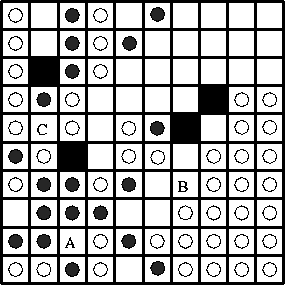
\includegraphics[scale=0.50]{stability.PNG}\\
Stable positions for white
\end{center}
\end{frame}

\begin{frame}{Piece Internality}
    \begin{itemize}
  \item
  A piece is internal if it has no empty neighbours
  \item
   Harder to dislodge, can result in higher mobility
  \end{itemize}
\end{frame}

\begin{frame}{Temporal Difference Learning}
   \begin{itemize}
  \item
  	Used a fairly standard TD($\lambda$) policy.
  \item
	Play whole game, recieve reward $r\in \left\{1,0,-1 \right\}$ for win/draw/loss.
  \item
	For each board $b_k$ position in the game, find the direction to adjust the weight in, based on making a small change and seeing if it improves/worsens the result.
 \item
	Then run through all of it is successors, and calculate the weighted difference between it's value and the successor's.
  \item
	$\sum_{t=k}^T \lambda^t \left ( V(b_t) - V(b_k) + feedback \right)$
  \end{itemize}
\end{frame}

\begin{frame}{Learning Strategies}
Josh to talk about this.\\
Alpha 0.01\\
E-greedy policy 0.15\\
\end{frame}

\begin{frame}{Negamax with alpha beta pruning}
    \begin{itemize}
  \item
    Adversarial search algorithm
  \item
    Minmax algorithm modified to negate the value at each step
  \item
    Attempts to maximise reward against adversary who is actively minimising reward
  \item
   $\alpha$ - $\beta$ pruning cuts sections of the game tree that an opponent would never choose
  \end{itemize}
\end{frame}

\begin{frame}{Negamax features}
    \begin{itemize}
  \item
    Search to a moderate depth if close to the start of the game
  \item
    Search to a deep depth if close to the end of the game
  \item
    Add depth if exploring along a forced move
  \item
    Use static evaluation feature weights to evaluate board value for us minus the board value for the opponent
  \item
    Terminals in our favour worth $\infty$, in opponent's favour worth $-\infty$.
  \end{itemize}
\end{frame}

\begin{frame}{Concurrency}
    \begin{itemize}
  \item
	Use concurrency to distribute MinMax search across multiple CPUs, thereby (hopefully) reducing the time taken for a search.
 \item
	Have to find a model of parallelism which balances putting processing time where it's needed vs overhead in communication between threads.
 \item
	We settled for a simplistic model - give each thread one of the 'top-level' MinMax nodes to search through. When it's done, give it another one.
 \item
	Has the downside that $\alpha \beta$ pruning data does not get updated until a thread finishes its node.
 \item
	Initial nodes can take more time than they otherwise might have.
 \item
	But still end up with an $O(n)$ speed up, where $n$ is the number of cores.
  \end{itemize}
\end{frame}

\begin{frame}{Time management}
    \begin{itemize}
  \item
    Lower depth based on amount of time left
  \item
    Emergency feature - Below 15 seconds, revert to depth 2 - we can see enemy moves as they come, but not much further ahead
  \end{itemize}
\end{frame}

\begin{frame}{Key Observations}
    \begin{itemize}
  \item
    Because of the removed squares, piece stability became especially important ahead
  \end{itemize}
\end{frame}

\begin{frame}{Other ideas}
    \begin{itemize}
  \item
    Use monte carlo prediction as a substitute for reward to help with learning of mid-game states
  \item
    Optimised search ordering - expand nodes by their value in our piece feature weights
  \end{itemize}
\end{frame}

\begin{frame}{Winning Speech}
    \begin{itemize}
  \item
    Friends, family, wives, pets, neighbours etc.
  \item
   Beyonce has one of the greatest videos of all time. Of all time!
  \item
   Other groups played well but we can't all be winners
  \end{itemize}
\end{frame}

\end{document} 
